\documentclass[12pt]{article}
\usepackage{../../includes/lecture_notes}
\usepackage{../../includes/math}
\usepackage{../../includes/uark_colors}
\hypersetup{
  colorlinks = true,
  allcolors = ozark_mountains,
  breaklinks = true,
  bookmarksopen = true
}
\begin{document}
\begin{center}
  {\Huge\bf Midterm - Spring 2025}
  
  \smallskip
  {\large\it ECON 5753 — University of Arkansas}
\end{center}

\medskip
\begin{enumerate}
  \item Say a researcher wants to model the conditional expectation of wages given gender, college degree, and age. The author includes a linear function of age, an indicator for having a college degree, and an indicator for being a female. Suggest a few (2 or 3) additional terms they could include in their model and give a reason why each term might be good to add. 

  \bigskip
  \item Say we have a survey of Americans (like the Current Population Survey). We run a \emph{linear regression} with having gone to college (taking values $0$ and $1$) on indicators for each race (White, Hispanic, Black, Native, and Asian/Pacific Islander). Here are the results:
  \begin{codeblock}[{}]
OLS estimation, Dep. Var.: has_college_experience
Observations: 226,666
Standard-errors: Heteroskedasticity-robust 
                                 Estimate Std. Error  t value  Pr(>|t|)    
(Intercept)                      0.716339   0.001187 603.5694 < 2.2e-16 ***
race::Asian or Pacific Islander  0.066815   0.003442  19.4098 < 2.2e-16 ***
race::Black                     -0.088041   0.003242 -27.1584 < 2.2e-16 ***
race::Hispanic                  -0.178127   0.002816 -63.2493 < 2.2e-16 ***
race::Native                    -0.167055   0.010281 -16.2492 < 2.2e-16 ***
---
Signif. codes:  0 '***' 0.001 '**' 0.01 '*' 0.05 '.' 0.1 ' ' 1
  \end{codeblock}

  \begin{enumerate}
    \item Interpret the coefficient on the Hispanic indicator. Comment on its statistical significance.
    
    \item We discussed in class concern about linear probablity model predicting fitted probabilities $\hat{\mathbb{P}}( Y_i = 1 \ | \ W_i = w )$ outside of $[0, 1]$. Does that problem come up in this model? Why or why not?
    
    \item What is the estimated difference in rates of having attended college between Hispanic and Native Americans. What would be a simple way to modify this regression to test significance of the difference? 
  \end{enumerate}

  \newpage
  \item You are analyzing a dataset of high-school basketball players. You have data on their physical attributes, their position played, and basic stats from their senior year. 
  \begin{enumerate}
    \item To flexibly model the relationship between points scored and height, you run a model with a 3rd-order polynomial. What concerns might you have with predicting the points scored for a high-school player who is 7'0''.
    
    % \item In class we discussed the concept of multivariable regression and ``all else equal''. Describe how your interpretation of a simple linear regression of points scored on height would change after adding a set of indicators for each position (point guard, shooting guard, small forward, power forward, and center).
    
    \item Say you want to let the relationship between height and points scored vary by position. Describe the regression you could run that would estimate different slopes by position, i.e. what terms would you include in your model?
  \end{enumerate}
    
  \bigskip
  \item A study analyzed a survey dataset of Americans aged 40-60. The surveys asked them how many drinks they have per week (options were 0, 1-3, 4-6, 7+) and health outcomes (e.g. an indicator for having cardiovascular problems).
  The study found that the compared to 0 drinks, the probability of having cardiovascular problems was 1.5\% lower for people who drank 1-3 drinks per week.
  \begin{enumerate}
    \item Explain what regression the researchers might have run to estimate this.
    
    \item Why might we be hesitant to not call this evidence the ``causal'' effect of having more drinks?
  \end{enumerate}

  
  \bigskip
  \item Two classmates are competing to find the best model to predict the winners of NFL games. Both train some kind of logistic regression model using a bunch of different variables with data on the past 3 seasons of games. They compare whose model performs better on their training sample and use the model that performs best. Why might this be a bad idea?

  \bigskip
  \item Figure \ref{fig:wage_vs_age} presents sample averages of a worker's income for each age (points).
  Additionally, the line presents fitted values from a regression of income on age and age$^2$.
  The regression results are shown below the figure. Answer the following questions:

  \begin{enumerate}
    \item True/False: the sample average for each bin gives an \emph{exact} estimate of the CEF.
    
    \item Predict someone's wage when they are 40 years old. Show your math if you do not have a calculator.
    
    \item What would be the change in wage predicted going from 30 to 31 years old? Show your math if you do not have a calculator. 
    
    \item Can you reject a linear relationship between age and income? Why or why not?
  \end{enumerate}

  \begin{figure}
    \caption{Sample average of wages for each age and a quadratic fit}
    \label{fig:wage_vs_age}
    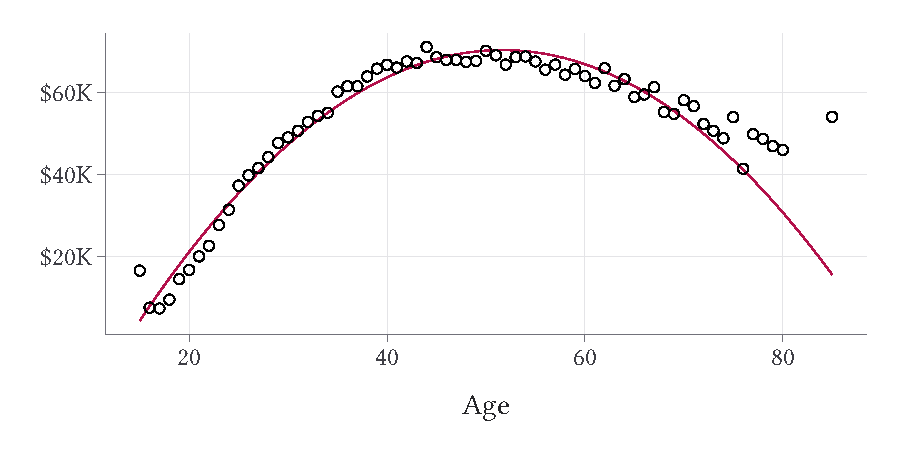
\includegraphics[width = \linewidth]{figures/plot_wage_age.pdf}
  \end{figure}

  \vspace*{-2\bigskipamount}
  \begin{codeblock}[{}]
OLS estimation, Dep. Var.: incwage
Observations: 226,666
Standard-errors: Heteroskedasticity-robust 
                Estimate  Std. Error  t value  Pr(>|t|)    
(Intercept) -60919.4890 1005.711304 -60.5735 < 2.2e-16 ***
age           5081.4608   54.379442  93.4445 < 2.2e-16 ***
I(age^2)       -49.2057    0.652094 -75.4579 < 2.2e-16 ***
---
Signif. codes:  0 '***' 0.001 '**' 0.01 '*' 0.05 '.' 0.1 ' ' 1
  \end{codeblock}


\end{enumerate}

\end{document}
